\subsection{Parameter Effects}
\label{sec:setup.char.paramfx}

In this section, we examine the effects of the parameters on the original model function.
We start with the combined parameter effects along a chain of parameter regions of the same period.
After that we will look into what role the parameters play individually.

\subsection{Combined Effects of Parameters}
\label{sec:setup.char.paramfx.combined}

To replicate the dynamics seen in the model, it is helpful to know, how the model changes along the \hl{chains of parameter regions that are associated with cycles of the same period}.
\hl{
	We therefore analyze the model function at different points in different chains.
}
\Cref{fig:setup.char.evolution.map} \hl{indicates the points used for this analysis}.
\Cref{fig:setup.char.evolution.12} shows, how the model function changes along the \hl{chain of parameter regions associated with cycles of} period 12.
In the figure, there are three functions \hl{$F^A, F^B,$ and $F^C$}.
\hl{
	The function $F^{A_{12}}$ is the model function with the parameters $E_0 = 15.9, \chi_0 = 0.11$.
}
\hl{These parameter values are marked with the point $A_{12}$ in} \Cref{fig:setup.char.evolution.map}.
\hl{
	The function $F^{B_{12}}$ is the model function with the parameters $E_0 = 17.07, \chi_0 = 0.182$.
	And the function $F^{C_{12}}$ is the model function with the parameters $E_0 = 18.5, \chi_0 = 0.27$.
}
\hl{Both the parameter values are marked accordingly in} \Cref{fig:setup.char.evolution.map}.

\begin{figure}
	\centering
	\begin{subfigure}{0.4\textwidth}
		\includegraphics[width=\textwidth]{99_Yunus/2D_Period_Zoomed_Effects/result.png}
		\caption{Points}
		\label{fig:setup.char.evolution.map}
	\end{subfigure}
	\begin{subfigure}{0.4\textwidth}
		\includegraphics[width=\textwidth]{99_Yunus/ParameterEffects/E0_hi_P12/illustration.png}
		\caption{Period 12}
		\label{fig:setup.char.evolution.12}
	\end{subfigure}
	\begin{subfigure}{0.4\textwidth}
		\includegraphics[width=\textwidth]{99_Yunus/ParameterEffects/E0_hi_P10/illustration.png}
		\caption{Period 10}
		\label{fig:setup.char.evolution.10}
	\end{subfigure}
	\begin{subfigure}{0.4\textwidth}
		\includegraphics[width=\textwidth]{99_Yunus/ParameterEffects/E0_hi_P08/illustration.png}
		\caption{Period 8}
		\label{fig:setup.char.evolution.08}
	\end{subfigure}
	\caption[Effects of parameters on the original model function]{
		The shapes of the original model function for different parameter values.
		(a) shows the points of the parameter values used for the other figures.
		Also, some chains are annotated with their period.
		(b) shows the evolution of the shape of the original model function along the chain of parameter regions with period 12 cycles.
		The blue function is the model function for the parameter values at point $A_{12}$, purple at point $B_{12}$, and red at point $C_{12}$.
		Here, blue is at point $A_{10}$, purple at point $B_{10}$, and red at point $C_{10}$.
		(c) shows the same thing for the chain of parameter regions with period 10.
		And (d) is for the chain of parameter regions with period 8.
		Here, blue is at point $B_8$ and red at point $C_8$.
		\todo{Label functions, update caption}
	}
	\label{fig:setup.char.evolution.combined}
\end{figure}

The most notable changes are \hl{the following}.
\begin{enumerate}
	\item The values of the \hl{whole} branches $F_\A$ and $F_\C$ get larger.
	      \hl{
		      This change is most notable at the left borders of the branches.
		      The values on the left sides of the branches are affected more by this change than the values on the right sides.
	      }
	\item \hl{
		      The values on the left sides of the branches $F_\B$ and $F_\D$ get smaller while the values on the right sides are not affected much.
	      }
	\item The local minima of \hl{the branches $F_\B$ and $F_\D$} move to the left, and their values get smaller.
\end{enumerate}
One smaller change is that the border between branches $F_\B$ and $F_\C$ moves left.
Note that the same change happens to the border between the branches $F_\D$ and $F_\A$ due to the symmetry of the function.

\hl{
	The same effects can be observed in the chains of parameter regions associated with cycles of periods $10$ and $8$, respectively.
}
\hl{For the chain of parameter regions associated with cycles of period $10$, the model function is plotted in} \Cref{fig:setup.char.evolution.10} \hl{at the three points $A_{10}, B_{10},$ and $C_{10}$ marked in} \Cref{fig:setup.char.evolution.map}.
\hl{
	Again, the values of the whole branches $F_\A$ and $F_\C$ are larger in $F^{C_{10}}$ than they are in $F^{A_{10}}$.
	And the values on the left sides of the branches $F_\B$ and $F_\D$ are smaller in $F^{C_{10}}$ than they are in $F^{A_{10}}$.
	Also, the local minima on those branches move left and down.
}
\hl{For the chain of parameter regions associated with cycles of period $8$, the model function is plotted in} \Cref{fig:setup.char.evolution.08} \hl{at the two points $B_8$ and $C_8$ marked in} \Cref{fig:setup.char.evolution.map}.
\hl{
	And the values of the branches undergo the same changes again from the model function $F^{B_8}$ to $F^{C_8}$.
}

\subsection{Individual Effects of Parameters}
\label{sec:setup.char.paramfx.individual}

The effects of the parameters described above, always include a change in both parameters $E_0$ and $\chi_0$.
To reproduce the bifurcation structures, it is important to know which effects on the function each parameter has individually.
\hl{
	We now fix one parameter and vary the other to observe the isolated effects of the varied parameter.
}

\begin{figure}
	\centering
	\includegraphics[width=0.4\textwidth]{99_Yunus/2D_Period_Zoomed_EffectsSingle/result.png}
	\caption[The parameter ranges examined to analyze the effects of parameters on the original model function]{
		The parameter ranges examined to analyze the effects of parameters $E_0$ and $\chi_0$ on the original model function
		The green arrow indicates the parameter range used for analyzing the effects of the parameter $E_0$, while the orange arrow indicates the parameter range used for analyzing the effects of the parameter $\chi_0$ on the original model function.
	}
	\label{fig:setup.char.evolution.single.map}
\end{figure}

For the \hl{effects of the} parameter $E_0$, we fix $\chi_0 = 0.2$ and vary $E_0$ in the parameter range $[15, 19]$.
This is marked as the green arrow in \Cref{fig:setup.char.evolution.single.map}.
As before, we plot the \hl{model} function at three \hl{parameter values} and put them in one figure.
\hl{The functions are visualized in} \Cref{fig:setup.char.evolution.e0}.
\hl{
	$F^L$ is the model function with $E_0 = 15$, $F^M$ is the model function with $E_0 = 17$, and $F^R$ is the model function with $E_0 = 17$.
	$\chi_0 = 0.2$ is the same for all functions $F^L, F^M,$ and $F^R$.
}
\hl{The parameter values are marked with the points $L, M,$ and $R$ in} \Cref{fig:setup.char.evolution.single.map}.
\hl{
	One can see that they are all on the green arrow mentioned before.
	The following changes can be observed.
}
\begin{enumerate}
	\item \hl{
		      The values on the left sides of the branches $F_\B$ and $F_\D$ get smaller while the values on the right sides are not affected much.
	      }
	\item The local minima of \hl{the branches $F_\B$ and $F_\D$} move left, and their values get smaller.
	\item The border between the branches $F_\A$ and $F_\B$ moves \hl{to the} right.
	      \hl{
		      The same is true for the border between the branches $F_\C$ and $F_\D$ because of the symmetry in the original model.
	      }
	\item The values at the right borders of branches $F_\A$ and $F_\C$ get larger. This is caused by the border between branches $F_\A$ and $F_B$ moving to the right.
\end{enumerate}

For the \hl{effects of the} parameter $\chi_0$, we fixed $E_0 = 17$ and varied $\chi_0$ in the parameter range $[0.125, 0.3]$.
This parameter range is marked with an orange arrow in \Cref{fig:setup.char.evolution.single.map}.
\hl{
	Again, we plot the model function at three parameter values and put them in one figure.
}
\hl{The functions are visualized in} \Cref{fig:setup.char.evolution.hi}.
\hl{
	$F^D$ is the model function with $\chi_0 = 0.1$, $F^M$ is the model function with $\chi_0 = 0.2$, and $F^U$ is the model function with $\chi_0 = 0.3$.
	$E_0 = 15$ is the same for all functions $F^D, F^M,$ and $F^U$.
}
\hl{The parameter values are marked with the points $D, M,$ and $U$ in} \Cref{fig:setup.char.evolution.single.map}.
\hl{
	One can see that they are all on the orange arrow mentioned before.
	The following pronounced changes can be observed.
}
\begin{enumerate}
	\item The values of the \hl{whole} branches $F_\A$ and $F_\C$ get larger.
	\item The border between the branches $F_\A$ and $F_\B$ moves to the left.
	      \hl{The same is true for the border between the branches $F_\C$ and $F_\D$}.
\end{enumerate}
\hl{
	Two other smaller changes that can be observed are the following.
}
\begin{enumerate}
	\item The values \hl{on the right sides} of the branches $F_\B$ and $F_\D$ get larger.
	      \hl{This includes the values of the local minima on these branches}.
	\item The border between the branches $F_\B$ and $F_\C$ moves to the left.
	      \hl{The same is true for the border between the branches $F_\D$ and $F_\A$}.
\end{enumerate}

\begin{figure}
	\centering
	\begin{subfigure}{0.4\textwidth}
		\includegraphics[width=\textwidth]{99_Yunus/ParameterEffects/E0/illustration.png}
		\caption{Parameter $E_0$}
		\label{fig:setup.char.evolution.e0}
	\end{subfigure}
	\begin{subfigure}{0.4\textwidth}
		\includegraphics[width=\textwidth]{99_Yunus/ParameterEffects/hi/illustration.png}
		\caption{Parameter $\chi_0$}
		\label{fig:setup.char.evolution.hi}
	\end{subfigure}
	\caption[The effects of single parameters on the original model function]{
		The effects of varying the parameters $E_0$ and $\chi_0$ alone on the original model function.
		(a) shows the effects of $E_0$ on the original model function.
		The red function is at the beginning of the parameter range depicted in \Cref{fig:setup.char.evolution.single.map}, purple is in the middle, and red is at the end.
		(b) shows the effects of $\chi_0$ on the original model function.
		Analogously to (a), the red function is at the beginning of the parameter range depicted in \Cref{fig:setup.char.evolution.single.map}, purple is in the middle, and red is at the end.
		\todo{Update caption}
	}
	\label{fig:setup.char.evolution.single}
\end{figure}

\subsection{Decomposition of Combined Effects}
\label{sec:yunus.param.effects.decomposition}

\hl{In this section, we take} a closer look at the combined effects of the parameters along \hl{chains of parameter regions associated with cycles of} the same period and trace them back to the isolated effects of \hl{either} parameter.
For this, we introduce a notation for the effects.
The effect of the values \hl{on the left side} of a branch changing is denoted $\AL$, for the \hl{right side} it is $\AR$, and for the whole branch it is $\AW$
The subscript indicates, which branch the change effects, and the superscript indicates, whether the values get larger $+$ or smaller $-$.
The effect of changing a local minimum is denoted as $\AMi$.
The meaning of the subscript stays the same as above, but the superscript also can include $L$ for \hl{movement to the left} and $R$ for \hl{movement to the right}.
Finally, the effect of moving borders is denoted as $\AB$.
The subscript now includes the two symbols of branches to which the border belongs and the superscript now has only $L$ or $R$.
For brevity, we do not write redundant branch names, so changes happening to branch $F_\A$ are also happening to branch $F_\C$.
For borders, changes to the border between branches $F_\A$ and $F_\B$ are also happening to the border between branches $F_\C$ and $F_\D$ and so on.

\Cref{table:setup.char.paramfx} lists all observed effects along the \hl{chains of parameter regions associated with cycles} of the same period and their decomposition into effects of the single parameters.
The first part of the table includes all major changes observed in \Cref{sec:setup.char.paramfx.combined}.
The second part includes the minor change one can observe of the borders between the branches $f_\B$ and $f_\C$ moving to the left.
The second part also includes the changes observed in \Cref{sec:setup.char.paramfx.individual} that cancel out.
From this table we can see, that $E_0$ causes the effects on the branches $F_\B$ and $F_\D$, while $\chi_0$ causes the changes to the branches $F_\A$ and $F_\C$, as well as the minor movement of the borders between the branches $F_\B$ and $F_\C$.
Note again, that the change to the border of branches $F_\B$ and $F_\C$ also applies for the border between branches $F_\D$ and $F_\A$.

\begin{table}
	\centering
	\begin{tabular}{|c|c|c|l|} \hline
		Combined         & $E_0$            & $\chi_0$          & Comment                   \\ \hline \hline
		$\AL_{\B}^{-}$   & $\AL_{\B}^{-}$   & 0                 & Only $E_0$ causes this    \\ \hline
		$\AMi_{\B}^{L-}$ & $\AMi_{\B}^{L-}$ & $-\AMi_{\B}^{+}$  &
		$E_0$ and $\chi_0$ have opposing effects, the effect of $E_0$ is stronger           \\ \hline
		$\AW_{\A}^{+}$   & 0                & $\AW_{\A}^{+}$    & Only $\chi_0$ causes this \\ \hline \hline
		$\AB_{\B\C}^{L}$ & 0                & $\AB_{\B\C}^{L}$  & Only $\chi_0$ causes this \\ \hline
		0                & $\AB_{\A\B}^{R}$ & $-\AB_{\A\B}^{L}$ &
		$E_0$ and $\chi_0$ have opposing effects, they cancel out                           \\ \hline
	\end{tabular}
	\caption[Decomposition table of combined parameter effects]{
		Decomposition of the combined parameter effects along chains of parameter regions with the same period as displayed in \Cref{fig:setup.char.evolution.combined}.
		Each effect is traced back to the effects of changing the parameters $E_0$ and $\chi_0$ alone as displayed in  \Cref{fig:setup.char.evolution.single}.
	}
	\label{table:setup.char.paramfx}
\end{table}
